\documentclass[12pt,a4paper]{article}
\usepackage[utf8]{inputenc}
\usepackage[german]{babel}
\usepackage[T1]{fontenc}
\usepackage{amsmath}
\usepackage{amsfonts}
\usepackage{amssymb}
\usepackage{graphicx}
\usepackage{siunitx}
\usepackage{float}
\usepackage[left=2cm,right=2cm,top=2cm,bottom=2cm]{geometry}
\author{Gerald}

\begin{document}
\sisetup{separate-uncertainty = true}
	\setlength{\parindent}{0pt} 
	\begin{center}
		{\LARGE Versuchsprotokoll}\\
		\begin{large}
			zum Fortgeschrittenenpraktikum im Bachelorstudiengang Physik\\[0.4cm]
			an der RWTH Aachen\\
			II. Physikalisches Institut A\\[5.5cm]
			\Large\textbf{\textsl{Mößbauerspektroskopie (T05)}}\\[5.5cm]
			\normalsize\textit{vorgelegt\\von}\\[0.4cm]
			\large{Moritz Berger (355244)\\Gerald Kolter (355005)}\\\textbf{Gruppe 30}\\[2cm]
			\large \textbf{Wintersemester 2017/18}
		\end{large}
	\end{center}
	\newpage
	
	\tableofcontents
	\newpage

\section{Versuchsziel}
Das Ziel des Versuchs besteht darin, mithilfe der Mößbauerlinie folgende quantenmechanische Energieaufspaltungen von Eisen zu vermessen:
\begin{enumerate}
\item Die magnetische Hyperfeinstruktur
\item Die elektrische Quadrupolaufspaltung
\end{enumerate}
Zudem soll die natürliche Linienbreite mithlife des Einlininespektrums von Eisen bestimmt werden und der Extinktionswirkungsquerschnitt von Eisen, Stahl und Eisensulfat vermessen werden.

\section{Aufbau und Funktion}
Der Aufbau zur Mößbauerspektroskopie besteht aus einer von einem Transducer in Strahlrichtung sinusförmig bewegten $^{57}$Co Quelle, einem Absorber und einem Detektor. Das Cobalt zerfällt in einen angeregten Eisenzustand, der dann $\gamma$-Strahlung von \SI{14,4}{keV},\SI{122}{keV} und \SI{136.5}{keV} aussendet, wobei hier hauptsächlich die \SI{14,4}{keV} Linie betrachtet wird. Mit einem eisenhaltigen Absorber, der zwischen Quelle und Detektor steht,können die $\gamma$-Quanten wieder absorbiert werden. Dies geschieht allerdings nur bei diskreten Energiewerten. Mithilfe des Transducers kann man die von der Quelle ausgesendete Strahlung durch den Doppler-Effekt um sehr kleine Energien verschieben. Dadurch verschiebt sich natürlich auch die Energie, die absorbiert werden muss, wodurch man sehr kleine Energieaufspaltungen untersuchen kann.\\
Als Detektor wird ein Proportionalzählrohr verwendet, durch welches die gemessenen Pulse nach ihrer Energie auf 1024 Channels verteilt wird.\\
Mithilfe eines Michelson-Interferometers, dass sich mit dem Transducer mitbewegt, kann über eine Kalibration aus den gemessenen Hell-Dunkel-Übergängen den Channels eine Momentangeschwindigkeit und somit eine Energieaufspaltung zugeordnet werden.

\section{Durchführung}

\begin{table}
\centering
\begin{tabular}{|c|c|}
\hline 
Spannung am Proportionalzählrohr & \SI{2}{kV} \\ 
\hline 
Messmodus & Pulshöhenanalyse (PHA-Modus) \\
\hline 
Messbereich im PHA-Modus & \SI{4,2}{V} - \SI{6,4}{V} \\
\hline 
\end{tabular} 
\caption{Allgemeine Messeinstellungen.}
\label{tab:Mess_Einstellungen}
\end{table}

Tabelle \ref{tab:Mess_Einstellungen} zeigt die verwendeten Messeinstellungen. Um bei für jede Messung den relevanten Energiebereich vermessen zu können, wurde die Transducer-Geschwindigkeit verändert.

\subsection{Kalibration}
Da der Detektor die gemessenen Zählraten in der Energie auf 1024 Kanäle aufteilt, muss eine Kalibration dieser Kanäle auf die Energie erfolgen. Dazu wird die Geschwindigkeit der Bewegung der Quelle mit einem Michelson-Interferometer gemessen und daraus über den Dopplereffekt die Energie der so verschobenen Linie berechnet. Diese Messungen wurden als Einzige mit dem Multi-Chanel-Scaler-Modus (MCS-Modus) aufgenommen. Diese Messung muss für jede neu eingestellte Transducer-Geschwindigkeit wiederholt werden. Für diese Messungen wurde der Timer, also die Messzeit, auf \SI{45}{s} gestellt.

\subsection{Untergrundmessung}
Um auf eine mögliche Nullrate korrigieren zu können, wird eine Messung ohne Quelle und ohne Absorber (mit leerem Absorberhalter) aufgenommen. Für die Aufnahme des Untergrunds wurde der Messbereich des PHA-Modus auf den maximal einstellbaren Bereich von \SI{10}{mv} - \SI{10}{V} eingestellt. Der Timer wurde auf \SI{10}{min} eingestellt.

\subsection{Quellenspektrum}
Für die Mößbauerspektroskopie muss zunächst die Mößbauerlinie gesucht werden. Dazu wird das gesamte Spektrum einmal mit großer und einmal ohne Bewegung der Quelle aufgenommen. Für die Aufnahme mit großer Geschwindigkeit wurde eine Bewegung von c.a 7 mm/s eingestellt. Dies wurde über eine Schnellauswertung mithilfe der Kalibration bestimmt. Für die Aufnahme des gesamten Quellspektrums wurde der Messbereich des PHA-Modus auf den maximal einstellbaren Bereich von \SI{10}{mV} - \SI{10}{V}. Das Quellspektrum wurde über eine Zeit von \SI{2}{min}. Der Mößbauerpeak sollte bei der Messung mit $v = \SI{0}{mm/s}$ schwächer ausfallen.

\subsection{Extinktionswirkungsquerschnitt}
Zur Bestimmung des Extinktionswirkungsquerschnitts $D_{ex}$ wird das Spektrum insgesamt vier mal aufgenommen:
\begin{enumerate}
\item Mit einem Stahl-Absorber
\item mit einem reinen Eisen-Absorber
\item mit einem FeSO$_4$ $\cdot$ 7H$_2$O-Absorber
\item ohne Absorber 
\end{enumerate} 
Um das gesamte Spektrum aufzunehmen, wurde der Messbereich auf \SI{10}{mV} - \SI{10}{V} gewählt. Jede dieser Messungen dauerte \SI{10}{min}. Der Extinktionswirkungsquerschnitt kann dann gemäß
\begin{equation}
D_{ex} = R(v) \cdot \dfrac{Z(v = \infty)}{Z(v)} = \dfrac{Z(v = \infty)}{Z(\textrm{ohne Absorber})}
\end{equation}
bestimmt werden, wobei Z die gesamte Zählrate ist. Für $v = \infty$ ist in der Realität eine Geschwindigkeit von wenigen mm/s ausreichend.

\subsection{Einlinienspektrum}
Das Einlinienspektrum wurde mit einem Absorber aus Stahl aufgenommen. Diese Messung lief \SI{1}{h}. Hier wurde eine Maximalgeschwindigkeit von c.a 3 mm/s eingestellt.

\subsection{Magnetische Hyperfeinstrukturaufspaltung}
Für die Vermessung der magnetischen Hyperfeinstrukturaufspaltung wurde das Spektrum mit einem Absorber aus reinem Eisen aufgenommen. Diese Messung lief über Nacht mit einer Gesamtmesszeit von \SI{18}{h}. Die Maximalgeschwindigkeit wurde auf c.a 6 mm/s eingestellt.


\subsection{Elektrische Quadrupolaufspaltung}
Für die Vermessung der elektrischen Quadrupolaufspaltung wird ein FeSO$_4$ $\cdot$ 7H$_2$O-Absorber verwendet. Hier ist im Gegensatz zu den anderen Messungen nur der Linienabstand und nicht die Linienform entscheidend. Diese Messung lief \SI{1}{h} \SI{45}{min} und mit einer Maximalbewegung von c.a 3 mm/s.
\newpage
\section{Ergebnisse}
\subsection{Kalibration}

\begin{figure}
\centering
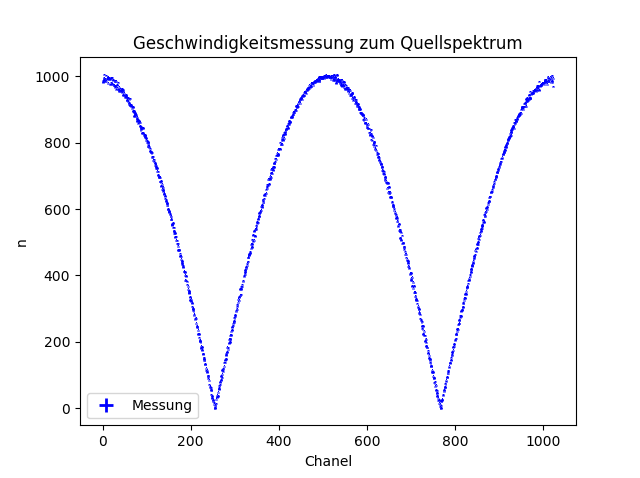
\includegraphics[scale=0.8]{Bilder/Kalibration/Quellspektrum_rohdaten.png}
\caption{Aufnahme zur Geschwindigkeits- und Energiekalibration vor der Messung des Quellspektrums.}
\label{fig:KalibrationRohdaten_Beispiel}
\end{figure}

\begin{table}
\centering
\begin{tabular}{|c|c|c|}
\hline 
Messung & Nulldurchgang 1 [ch] & Nulldurchgang 2 [ch] \\ 
\hline 
Extinktionswirkungsquerschnitt & 255 & 767 \\
\hline 
Quellspektrum & 255 & 767 \\
\hline 
Einlinienspektrum & 256 & 766 \\
\hline 
Hyperfeinstrukturaufspaltung & 255 & 766 \\
\hline 
Quadrupolaufspaltung & 255 & 767 \\
\hline 
\end{tabular} 
\caption{Abgelesene Nulldurchgänge bei den Geschwindigkeitsmessungen.}
\label{tab:Kalibration_Nulldurchgänge}
\end{table}

Abbildung \ref{fig:KalibrationRohdaten_Beispiel} zeigt beispielhaft das Messergebnis zur Geschwindigkeitsmessung. Da der Transducer die Quelle sinusförmig bewegt und die Messung der Hell-Dunkel-Übergänge nur Beträge und keine Vorzeichen misst, handelt es sich um eine Kosinus-Betragsfunktion. Für die Kalibration wird allerdings die reine Kosinusfunktion benötigt, daher werden die Daten zwischen den Nulldurchgängen mit (-1) multipliziert. Die zu diesem Zweck abgelesenen Nulldurchgänge sind in Tabelle \ref{tab:Kalibration_Nulldurchgänge} aufgelistet. \\
An die so korrigierten Daten wird dann eine Kosinusfunktion der Form
\begin{equation*}
n(\textrm{ch}) = A \cdot \cos (\omega \cdot \textrm{ch})
\end{equation*}
angepasst. Als Fehler für die Anpassung wurde für die Kanalaufteilung eine Gleichverteilung zwischen den Kanälen angenommen. Für den Fehler auf die counts wurde ein möglichst kleiner Wert verwendet, für den der Fit immer noch stabil ist. Für die Anpassungen wurden daher folgende Fehler verwendet:
\begin{equation*}
\sigma _{counts} = 2
\end{equation*}
\begin{equation*}
\sigma _\textrm{ch} = \dfrac{1}{\sqrt{12}}
\end{equation*}
Die korrigierten Daten und die Anpassung sind für dasselbe Beispiel in Abbildung \ref{fig:Kalibration_Beispiel} gezeigt. Die Ergebnisse der Anpassungen sind in Tabelle \ref{tab:Kalibration_Fitergebnisse} dargestellt. \\
Aus der Anpassung kann die dem Kanal zugehörige Momentangeschwindigkeit und daraus mit dem Dopplereffekt die Energie bestimmt werden:
\begin{equation*}
v(\textrm{ch}) = \dfrac{n(\textrm{ch}) \cdot 1024}{3160.56 \cdot t \textrm{[s]}} \, \textrm{[mm/s]}
\end{equation*}
Wobei die Hell-Dunkel-Wechsel $n(\textrm{ch})$ aus der Anpassung bestimmt werden.
\begin{equation*}
E(v) = E_0 \cdot \left(1 + \dfrac{v}{c}\right)
\end{equation*}
Wobei $E_0 = \SI{14,4}{keV}$ die Energie der verwendeten Linie ist. Die Fehler aus den Anpassungen pflanzen sich gaußisch auf die Geschwindigkeit und die Energie fort.\\
Aus der Amplitude kann man die maximale Geschwindigkeit und Energie und somit den Messbereich bestimmen. Die Ergebnisse sind in Tebelle \ref{tab:kal} aufgelistet.



\begin{table}
\centering
\begin{tabular}{|c|c|c|c|}
\hline 
Messung & Amplitude A & Frequenz $\omega$ & $\chi ^2$/ndof \\ 
\hline 
Extinktionswirkungsquerschnitt & 1053,28 $\pm$ 0,30 & 0,00615017 $\pm$ 5,7 $\cdot 10^{-7}$ & 9,394  \\
\hline 
Quellspektrum & 994,96 $\pm$ 0,29 & 0,00615257 $\pm$ 5,8 $\cdot 10^{-7}$ & 8,918 \\
\hline 
Einlinienspektrum & 387,30 $\pm$ 0,22 & 0,0061532 $\pm$ 1,0 $\cdot 10^{-6}$ & 5,768  \\
\hline 
Hyperfeinstrukturaufspaltung & 790,01 $\pm$ 0,29 & 0,00615317 $\pm$ 7,0 $\cdot 10^{-7}$ & 9,554  \\
\hline 
Quadrupolaufspaltung & 471,48 $\pm$ 0,18 & 0,00615197 $\pm$ 6,8 $\cdot 10^{-7}$ & 3,835 \\
\hline 
\end{tabular} 
\caption{Ergebnisse der Anpassungen an die Daten der Kalibrationsmessungen.}
\label{tab:Kalibration_Fitergebnisse}
\end{table}

\begin{table}
\centering
\begin{tabular}{|c|c|c|}
\hline 
Messung & Geschwindigkeitsbereich[mm/s] & Energiebereich[neV] \\ 
\hline 
Extinktionswirkungsquerschnitt &$\pm7.583 \pm 0.002 $ & $\pm 364.0 \pm 0.1 $\\
\hline 
Quellspektrum & $\pm 7.164 \pm 0.002 $ & $\pm 343.8 \pm 0.1 $\\
\hline 
Einlinienspektrum & $\pm 2.788 \pm 0.002 $ & $\pm 133.8 \pm 0.1 $\\
\hline 
Hyperfeinstrukturaufspaltung & $\pm 5.688 \pm 0.002 $ & $\pm 273.0 \pm 0.1 $\\
\hline 
Quadrupolaufspaltung & $\pm 3.395 \pm 0.001 $ & $\pm 162.9 \pm 0.1 $\\ 
\hline 
\end{tabular}
\caption{Messbereiche, die sich aus der Kalibration ergeben. Der Energiebereich gibt die Abweichung von $E_0 = \SI{14,4}{keV}$ an.}
\label{tab:kal}
\end{table}

\begin{figure}
\centering
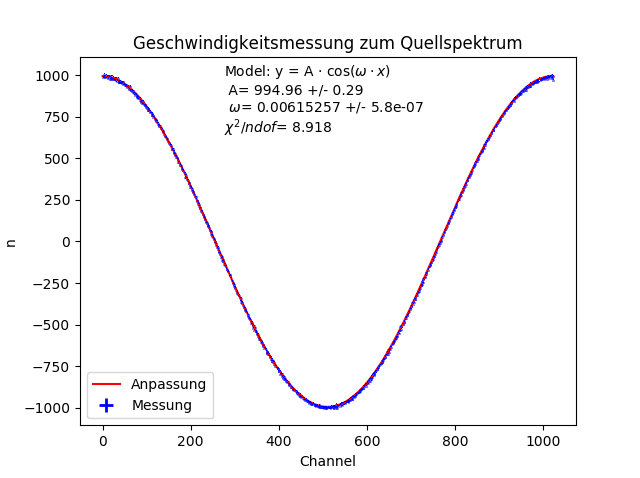
\includegraphics[scale=0.8]{Bilder/Kalibration/Quellspektrum.png}
\caption{Aufnahme zur Geschwindigkeits- und Energiekalibration vor der Messung des Quellspektrums.}
\label{fig:Kalibration_Beispiel}
\end{figure}

\subsection{Untergrundmessung}
\begin{figure}
\centering
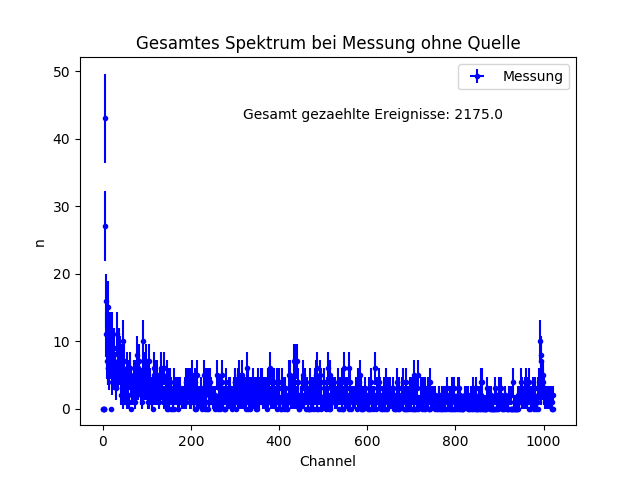
\includegraphics[scale=0.8]{Bilder/Extinktion/Rauschmessung.png}
\caption{Untergrundmessung ohne Quelle und ohne Absorber zur Korrektur bei den Messungen zum Extinktionswirkungsquerschnitt.}
\label{fig:Extinktion_Rauschmessung}
\end{figure}

Abbildung \ref{fig:Extinktion_Rauschmessung} zeigt das ohne Quelle und ohne Absorber gemessene Spektrum. Da es sich bei den gemessenen Ereignissen um Zerfälle handelt ist der Fehler darauf die Wurzel:
\begin{equation*}
\sigma _{n} = \sqrt{n}
\end{equation*}
Die Gesamtzahl der gemessenen Ereignisse ist:
\begin{equation*}
Z_{Untergrund} = \dfrac{2175 \pm 47}{\SI{10}{min}}
\end{equation*}

\subsection{Quellenspektrum}
\begin{figure}
\centering
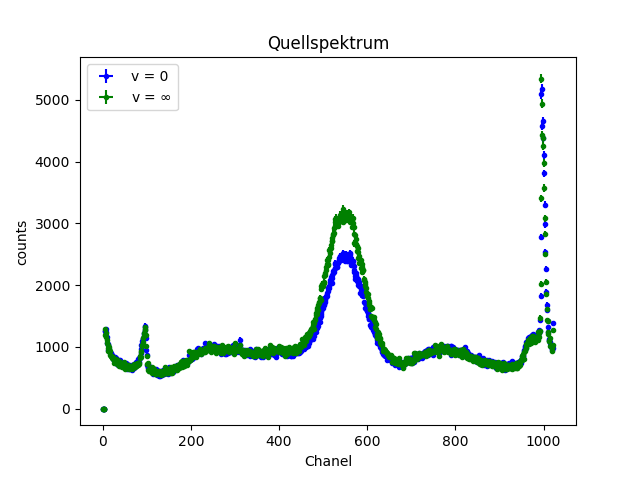
\includegraphics[scale=0.8]{Bilder/Quellspektrum/v0_und_vinf.png}
\caption{Gemessenes Quellspektrum.}
\label{fig:Quellspektrum}
\end{figure}

Abbildung \ref{fig:Quellspektrum} zeigt die Messungen des Quellspektrums für Transducergeschwindigkeit $v = 0$ und $v = \infty$ übereinandergelegt (wobei für $v = \infty$ in der Praxis einige mm/s eingestellt wurde). Durch das Übereinanderlegen der beiden gemessenen Spektren ist der Mößbauerpeak deutlich zu erkennen, da dies die einzige Stelle des Spektrums ist, bei der die beiden Messergebnisse voneinander abweichen. Für die folgenden Vermessungen der Energieaufspaltungen wurde daher in diesen Peak reingezoomt.\\
Für eine grobe Kanal-Energie-Kalibrierung können der Mößbauerpeak ($E_{Moessbauer} = \SI{14,4}{keV}$) und der scharfe Peak links verwendet werden, bei dem es sich um die $K_{\alpha}$-Linie von Eisen bei etwa $E_{K_{\alpha}} = \SI{7,1}{keV}$ handelt. Die abgelesenen Peakpositionen sind:
\begin{equation*}
\textrm{ch} _{K_{\alpha}} = 97 \quad \textrm{und} \quad \textrm{ch} _{Moessbauer} = 546 
\end{equation*}
Sodass sich unter Annahme eines linearen Zusammenhangs zwischen Energie und Kanal
\begin{equation*}
E = a \cdot \textrm{ch} + b
\end{equation*}
die Parameter ergeben zu:
\begin{equation*}
a = \SI{0,0163}{keV/ch} \qquad b = \SI{5,5}{keV}
\end{equation*}
Der scharfe Peak rechts im Spektrum, der abgelesen ca. bei Kanal 996 liegt, liegt damit bei einer Energie von ca. \SI{21,7}{keV}. Diesen Peak konnten wir nicht zuordnen. Die Photopeaks von Cobalt liegen bei \SI{14,4}{keV}, \SI{121,9}{keV} und \SI{136,3}{keV}. Die zugehörigen Compton-Kanten bei \SI{0,8}{keV}, \SI{39,4}{keV} und \SI{47,4}{keV}, die Rückstoßpeaks entsprechend bei \SI{13,2}{keV}, \SI{82,5}{keV} und \SI{88,9}{keV}. Diese Phänomene können den Peak also nicht erklären. Fremdstrahlung, also $\gamma$-Strahlung aus einer anderen Quelle, kann es auch nicht sein, denn dann hätte man den Peak in der Untergrundmessung auch sehen müssen.  


\subsection{Extinktionswirkungsquerschnitt}
\begin{figure}
\centering
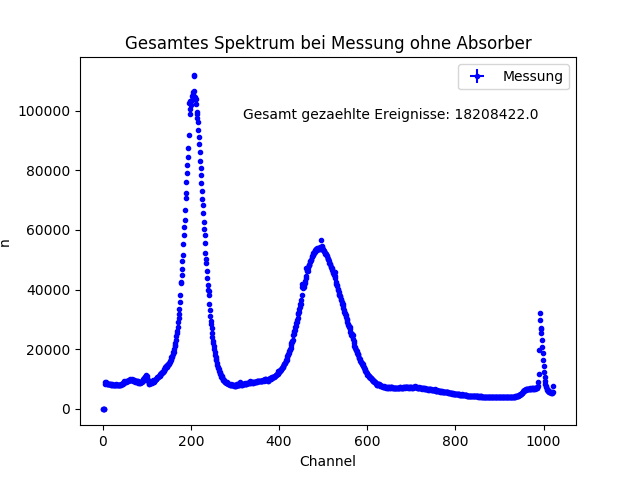
\includegraphics[scale=0.8]{Bilder/Extinktion/OhneAbsorber.png}
\caption{Messung ohne Absorber zur Bestimmung des Extinktionswirkungsquerschnitt.}
\label{fig:Extinktion_ohneAbsorber}
\end{figure}

\begin{figure}
\centering
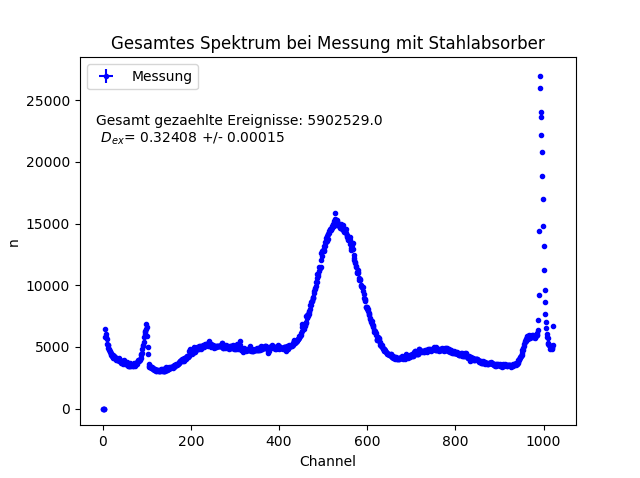
\includegraphics[scale=0.8]{Bilder/Extinktion/Stahl.png}
\caption{Messung mit Stahlabsorber zur Bestimmung des Extinktionswirkungsquerschnitts von Stahl.}
\label{fig:Extinktion_Stahl}
\end{figure}

Abbildung \ref{fig:Extinktion_ohneAbsorber} zeigt das gemessene Spektrum ohne Absorber und Abbildung \ref{fig:Extinktion_Stahl} beispielhaft für die Messung mit dem Stahlabsorber. \\
Da die Messungen des Untergrunds, die Messung ohne Absorber und die Messungen mit den Absorbern alle gleich lang sind, kürzt sich die Messzeit bei der Berechnung des Extinktionswirkungsquerschnitts raus, sodass es ausreicht die Ereigniszahl zu betrachten.\\ 
Zur Bestimmung des Extinktionswirkungsquerschnitts wird die Zählrate des gesamten Spektrums integriert bzw. wegen der Kanalauflösung aufsummiert. Auch hier wird der Fehler als 
\begin{equation*}
\sigma _{n} = \sqrt{n}
\end{equation*}
abgeschätzt. Zur Berechnung des Extinktionswirkungsquerschnitts müssen sowohl die Zählrate mit dem jeweiligen Absorber $n_A$ als auch die Zählrate ohne Absorber $n_O$ um die Untergrundmessung $n_U$ korrigiert werden, sodass sich der Extinktionswirkungsquerschnitt insgesamt bestimmt zu:
\begin{equation*}
D_{ex} = \dfrac{n_A - n_U}{n_O - n_U}
\end{equation*}
Damit bestimmt sich der Fehler mit gaußscher Fehlerfortpflanzung und der Annahme, dass die Fehler auf die Zählraten immer die Wurzel der Zählraten sind:
\begin{equation*}
\sigma _{D_{ex}} = D_{ex} \cdot \sqrt{ \left( \dfrac{\sqrt{n_O + n_U}}{n_O - n_U} \right)^2 +  \left( \dfrac{\sqrt{n_A + n_U}}{n_A - n_U} \right)^2}
\end{equation*}
Tabelle \ref{tab:Extinktion_Ergebnisse} zeigt die gemessenen Zählraten und die daraus berechneten Extinktionswirkungsquerschnitte.

\begin{table}
\centering
\begin{tabular}{|c|c|c|}
\hline 
Absorber & Zählrate $n_A$ & Extinktionswirkungsquerschnitt $D_{ex}$ \\ 
\hline 
Stahl & 5902529 & 0,32408 $\pm$ 0,00015 \\
\hline 
Reines Eisen & 5746105 & 0,31549 $\pm$ 0,00015 \\
\hline
Eisensulfat & 7385135 & 0,40552 $\pm$ 0,00018 \\
\hline
\end{tabular} 
\caption{Gemessene Zählraten und daraus berechnete Extinktionswirkungsquerschnitte.}
\label{tab:Extinktion_Ergebnisse}
\end{table}

Vergleicht man das Spektrum ohne Absorber (Abb. \ref{fig:Extinktion_ohneAbsorber}) und das Spektrum mit Absorber (bspw. Abb. \ref{fig:Extinktion_Stahl}), fallen folgende Dinge auf:
\begin{enumerate}
\item Der breite Peak bei ca. Chanel 500 behält mit Einfügen eines Absorbers seine Form, die Höhe wird nur geringer
\item Der scharfe Peak bei ca. Chanel 1000 bleibt mit Einfügen eines Absorbers in Form und Höhe unverändert
\item Im Spektrum ohne Absorbers gibt bei ca. Chanel 200 einen scharfen Peak, der in den Spektren mit Absorber gar nicht zu sehen ist
\end{enumerate}
Diese Phänomene werden einzeln betrachtet:
\begin{enumerate}
\item Ein Abschwächen der Strahlung mit Einfügen eines Absorbers ist erwartet, auch dass die Form der Peaks dabei gleich bleibt
\item Der Peak, der in Form und Höhe unverändert bleibt, taucht in der Untergrundmessung nicht auf, d.h. es handelt sich um Strahlung, die von der Quelle kommt und unverändert durch alle drei Absorber geht. Wie das genau zustande kommt, ist unklar
\item Der Peak, der nur in dem Spektrum ohne Absorber zu sehen ist, stammt vermutlich von der Elektronen-Strahlung aus der Inneren Konversion. Ein solcher müsste knapp unter dem Mößbauerpeak liegen, da die kinetische Energie dieser Elektronen der Differenz zwischen der Energie des Mößbauerpeaks und der Bindungsenergie des Hüllenelektrons entspricht
\end{enumerate}


\subsection{Einlinienspektrum}

\subsubsection{Linienbreite}
\begin{figure}
\centering
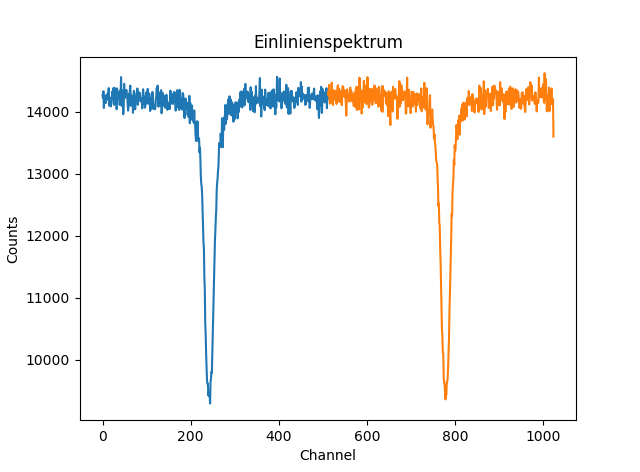
\includegraphics[scale=0.8]{Bilder/Einlinien/Ein_Rohdaten.png}
\caption{Messrate aufgetragen gegen den Channel.}
\label{fig:Ein_Roh}
\end{figure}

\begin{figure}
\centering
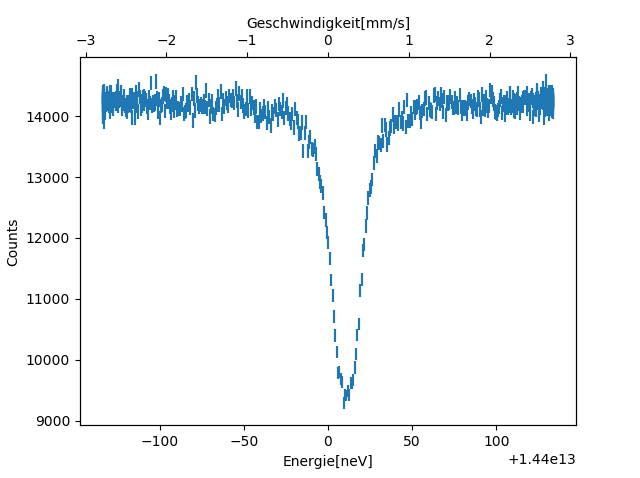
\includegraphics[scale=0.49]{Bilder/Einlinien/Ein_Data_vor.png}
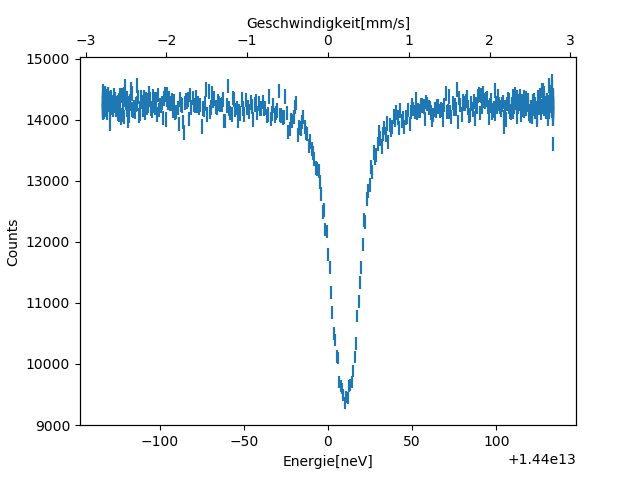
\includegraphics[scale=0.49]{Bilder/Einlinien/Ein_Data_nach.png}
\caption{Counts des Einlinienspektrums aufgetragen gegen Geschwindigkeit und Energie.}
\label{fig:Ein_Data}
\end{figure}

\begin{figure}
\centering
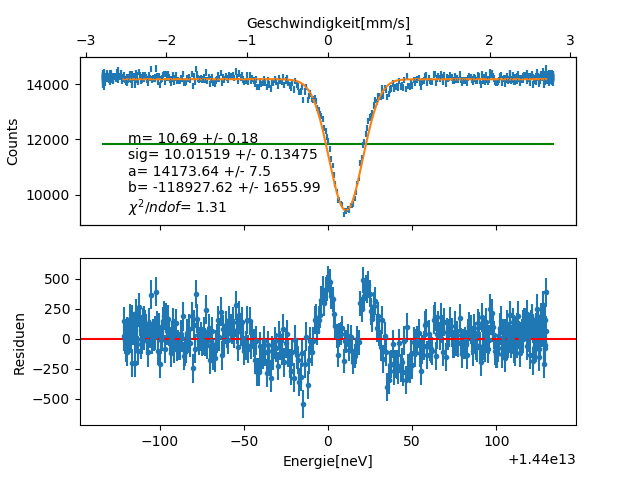
\includegraphics[scale=0.8]{Bilder/Einlinien/Ein_gauss_vor.png}
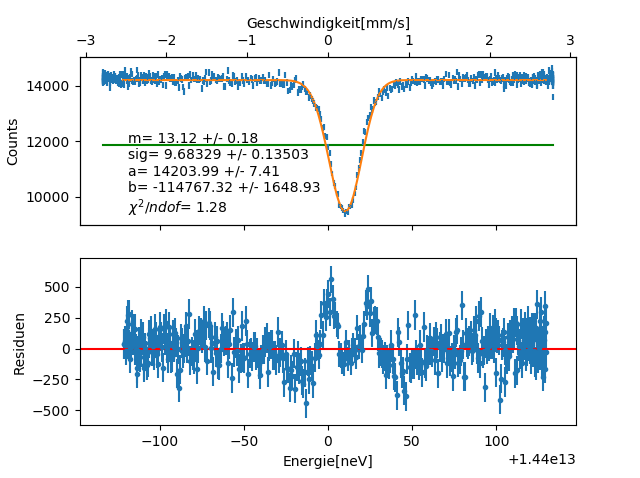
\includegraphics[scale=0.8]{Bilder/Einlinien/Ein_gauss_nach.png}
\caption{Counts des Einlinienspektrums aufgetragen gegen Geschwindigkeit und Energie.}
\label{fig:Ein_gauss}
\end{figure}

\begin{figure}
\centering
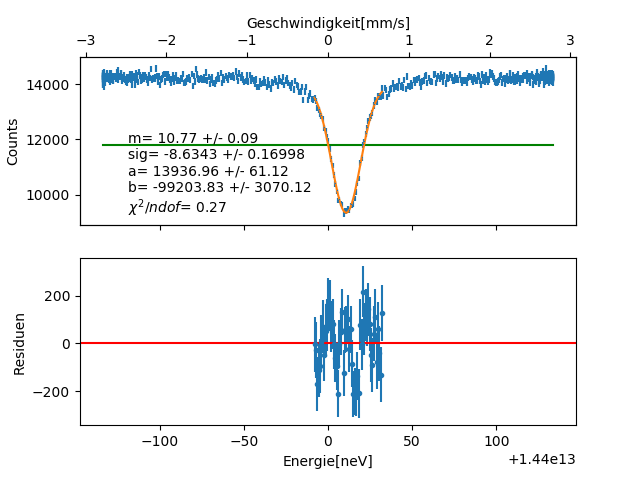
\includegraphics[scale=0.8]{Bilder/Einlinien/Ein_halbgauss_vor.png}
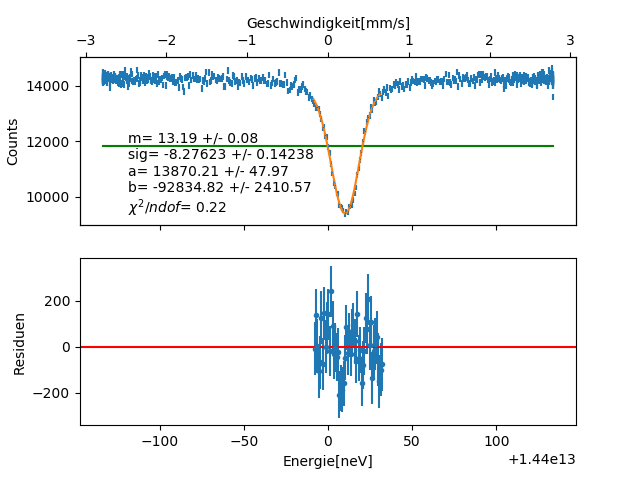
\includegraphics[scale=0.8]{Bilder/Einlinien/Ein_halbgauss_nach.png}
\caption{Anpassung von Gausspeaks an die }
\label{fig:Ein_halbgauss}
\end{figure}

In Abbildung \ref{fig:Ein_Roh} sind die Rohdaten der Vermessung des Einlinienspektrums dargestellt.\\
Da sich der Tranducer vor und zurück bewegt wiederholt sich das Spektrum in der hinteren Hälfte der Channel. Die vordere Hälfte beschreibt eine Schwingung von maximal negativer Geschwindigkeit bis maximal positiver, während die hintere Hälfte genau andersrum verläuft.\\
Kalibriert man nun die Channels gegen Geschwindigkeit und Energie nach Kapitel TBD, so ergeben sich aus den beiden Hälften 2 Spektren, die das selbe beschreiben. Diese werden im folgenden beide getrennt ausgewertet, um das Ergebnis am Ende zu mitteln.\\
Abbildung \ref{fig:Ein_Data} zeigt beide Spektren. Da es sich hier um radioaktive Zerfälle handelt, welche einer Poisson-Verteilung folgen, wird der Fehler auf die Counts mit $\sqrt{N}$ angenommen, wobei N die Anzahl der Counts darstellt. Aus der Kalibration erhält man außerdem einen Fehler in x-Richtung. Dieser ist aber um ein vielfaches kleiner als der Fehler auf die Counts, weswegen er nicht mit ins Gewicht fällt.\\
\\
Um die Eigenschaften der Peaks untersuchen zu können wird nun ein Gaussfit an diese angepasst. An diesen sollte man die Peakposition und über die Standardabweichung $\sigma$ mithilfe von 
\begin{equation}
\Gamma = 2\sqrt{2\log(2)}\sigma
\end{equation}
die Linienbreite $\Gamma$  bestimmtn können. Die Ergebnisse sind in Tabelle \ref{tab:Ein_gauss} zusammengefasst. Die Fehler werden direkt aus der Anpassung gaussisch fortgepflanzt.\\

\begin{table}
\centering
\begin{tabular}{|c|c|c|c|}
\hline 
Bereich & Peakposition [neV] & Linienbreite über Höhe [neV] & Linienbreite über $\sigma$ [neV]\\ 
\hline 
vorne & $10.69\pm 0.18$ & $23.82^{+0.05}_{-0.06}$ & $23.58\pm 0.32$ \\ 
\hline 
hinten & $13.12\pm 0.18$ & $22.92\pm 0.06$ & $22.80\pm 0.32$ \\ 
\hline 
\end{tabular}
\caption{Ergebnisse der Gaussanpassung an den ganzen Peak.}
\label{tab:Ein_gauss}
\end{table}

Unter Annahme eines perfekten Gausspeaks, dessen Anpassung in Abbildung \ref{fig:Ein_gauss} gezeigt ist, zeigt sich aber, dass der Peak nach untenhin breiter als die Anpassung wird und somit das Ergebnis nicht sehr genau ist.\\
Dies sieht man vorallem an der Systematik in den Residuen im relevanten Bereich.\\
\\
Deswegen wird stattdessen die Anpassung nur an der Spitze durchgeführt. Dies ist in Abbildung \ref{fig:Ein_halbgauss} zu sehen.\\
Diese Anpassung repräsentiert allerdings nur die Position des Peaks. Um trotzdem die Halbwertsbreite bestimmen zu können wird eine Rauschmessung an einem Ausschnitt der ebenen Daten durchgeführt. Diese ist in Abbildung \ref{fig:Ein_Rausch} dargestellt.\\
Mithilfe von 
\begin{equation}
h = N_0 - \dfrac{N_0-N_P}{2} = \dfrac{N_0+N_P}{2}
\end{equation}
ergibt sich schließlich die Position der halben Höhe des Peaks. Dabei ist $N_0$ der Mittelwert der Rauschmessung, also die Referenzhöhe, und $N_P$ die Höhe des Peaks.\\
Der Fehler auf die Halbhöhe ergibt sich aus gausscher Fehlerfortpflanzung der Fehler von Mittelwert und Peakposition.\\
Die Halbwertsbreite wird nun über die Schnittpunkte der Anpassung mit der Halbhöhe bestimmt. Der Fehler der Halbwertsbreite ergibt sich über die Verschiebemethode. Dabei wird die Anpassung um ihre Fehler (in allen Kombinationen) verschoben und eine neue Halbhöhe und neue Halbwertsbreite ausgerechnet. Aus der maximalen Abweichung vom Ursprünglichen Wert erhält man dann den Fehler.\\
\\
Die x-Position des Peaks erhält man weiterhin direckt aus der Anpassung.\\
Alle Ergebnisse sind in Tabelle \ref{tab:Ein_halbgauss} zusammengefasst.\\
Eine gewichtete Mittelung der über die Höhe bestimmte Linienbreite ergibt das Endergebnis:
\begin{equation*}
\boxed{\Gamma = \SI{20.95\pm 0.32}{neV}}
\end{equation*}

\subsubsection{Isomerieverschiebung}
Aus der Abweichung der Peaklage von der Null-Energie erhält man außerdem die Isomerieverschiebung. Auch die Peaklage wird gemittelt und man erhält:
\begin{equation*}
\boxed{\delta = \mu = \SI{12.08\pm 1.17}{neV}}
\end{equation*}

\begin{table}
\centering
\begin{tabular}{|c|c|c|c|}
\hline 
Bereich & Peakposition [neV] & Linienbreite über Höhe [neV] & Linienbreite über $\sigma$ [neV]\\ 
\hline 
vorne & $10.77\pm 0.09$ & $21.31^{+0.23}_{-0.25}$ & $20.33\pm 0.40$ \\ 
\hline 
hinten & $13.19\pm 0.08$ & $20.66 \pm 0.22$ & $19.49\pm 0.34$ \\ 
\hline 
\end{tabular}
\caption{Ergebnisse der Gaussanpassung an die Spitze des Peaks.}
\label{tab:Ein_halbgauss}
\end{table}

\begin{figure}
\centering
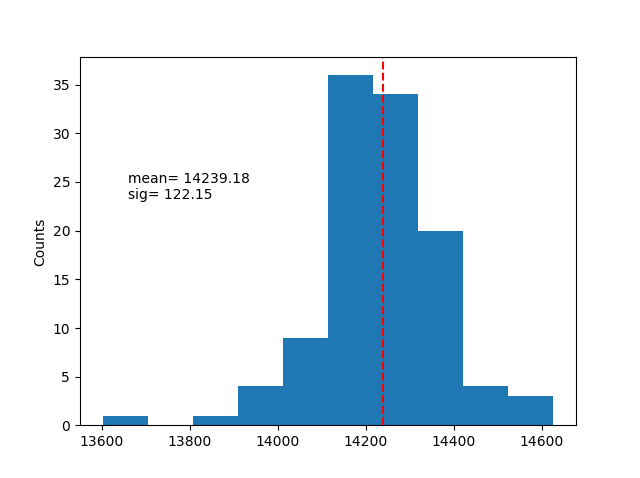
\includegraphics[scale=0.49]{Bilder/Einlinien/Ein_Rausch.png}
\caption{Rauschmessung zur bestimmung der Höhe}
\label{fig:Ein_Rausch}
\end{figure}

\subsubsection{Vergleich mit Literaturwerten}
Die berechnete Linienbreite entspricht noch nicht der natürlichen Linienbreite, sondern
\begin{equation}
\Gamma = (2+0.27\beta f' d n \sigma_0) \cdot \Gamma_{nat} = const \cdot \Gamma_{nat}
\end{equation}
mit $\beta = 0.022$,$f' = 0.85$,$d = 25\mu m$ und $n=8.4\cdot 10^{22}cm^{-3}$, wobei 
\begin{equation}
\sigma_0 = 2 \pi \dfrac{c^2 \hbar^2}{E_0^2} \dfrac{1}{1+\alpha} \dfrac{2 J_a+1}{2 J_g+1} \approx 2.38\cdot 10^{-22} m^2
\end{equation}
mit $E_0 = 14.4keV$, $\alpha = 8.9$,$J_a = 3/2$,$J_g = 1/2$. Darasu folgt 
\begin{equation}
const \approx 4.527
\end{equation}
Damit folgt die berechnete Natürliche Linienbreite und über
\begin{equation}
\tau_{exp} = \dfrac{\hbar}{\Gamma_{nat}}
\label{eq:tau}
\end{equation}
die berechnete Lebensdauer. Alle Fehler werden gaußisch fortgepflanzt.\\
\\
Die erwartete Lebensdauer berechnet sich über die Halbwertszeit:
\begin{equation}
\tau_{theo} = \dfrac{\hbar\cdot ln(2)}{T_{1/2}}
\end{equation}
woraus man über Gleichung \ref{eq:tau} dei erwartete Linienbreite bekommt.

\begin{table}
\centering
\begin{tabular}{|c|c|c|c|}
\hline 
 & echte Linienbreite[neV] & nat. Linienbreite[neV] & Lebensdauer[ns]\\ 
\hline 
Gemessen & $20.95\pm 0.32$ & $4.63\pm 0.07$ & $142.22\pm2.16$\\ 
\hline 
Erwartung & 21.08 & 4.66 & 141.38\\ 
\hline 
\end{tabular} 
\label{tab:Ein_lit}
\caption{Alle Ergebnisse der Messung und erwartete Werte.}
\end{table}


\subsection{Magnetische Hyperfeinstrukturaufspaltung}

\subsubsection{Magentfeldstärke}

\begin{figure}
\centering
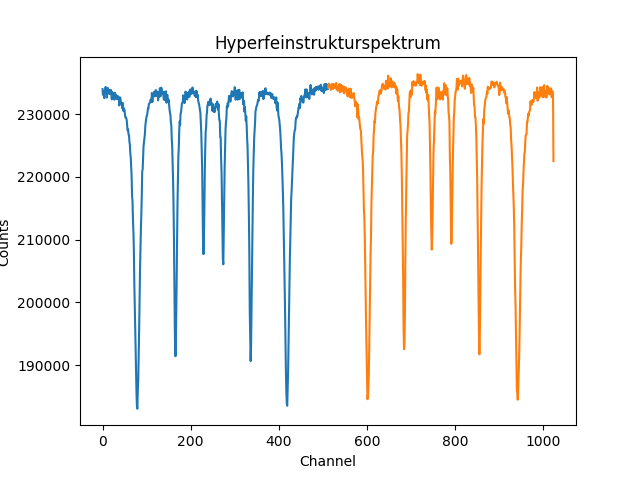
\includegraphics[scale=0.8]{Bilder/Hyperfein/Hyper_Roh.png}
\caption{Hyperfeinstrukur Rohdaten}
\label{fig:Hyper_Roh}
\end{figure}

\begin{figure}
\centering
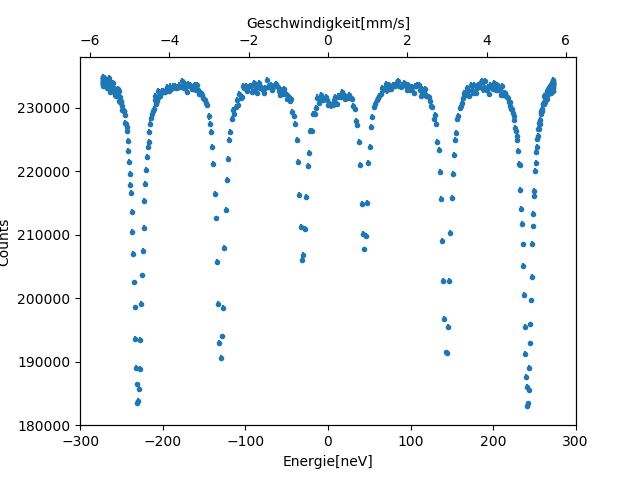
\includegraphics[scale=0.8]{Bilder/Hyperfein/Hyper_Data_vor.png}
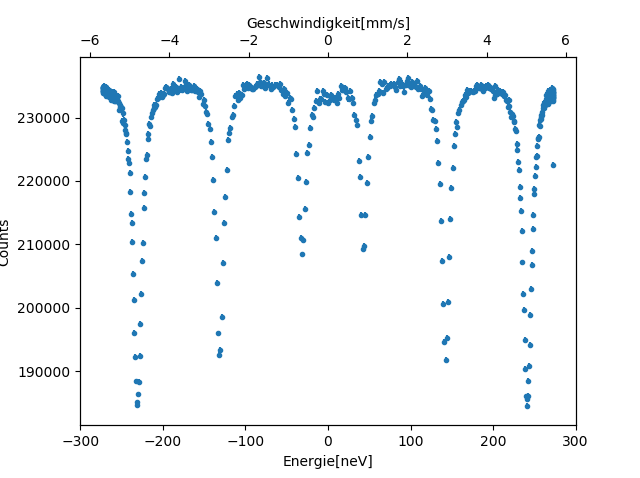
\includegraphics[scale=0.8]{Bilder/Hyperfein/Hyper_Data_nach.png}
\caption{Hyperfeinstrukur Counts gegen Geschwindigkeit und Energie aufgetragen.}
\label{fig:Hyper_Data}
\end{figure}

\begin{figure}
\centering
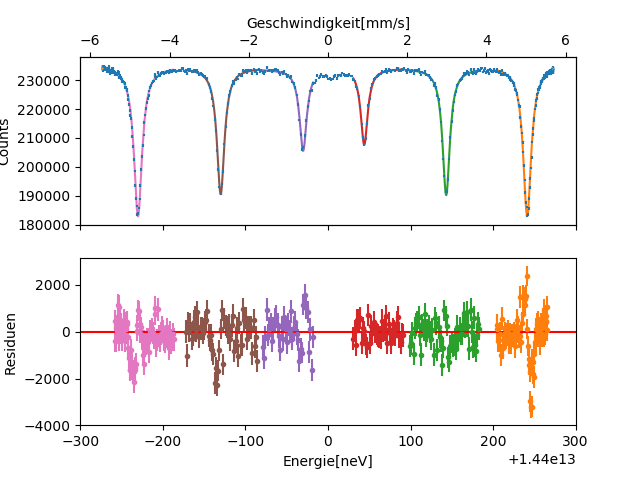
\includegraphics[scale=0.9]{Bilder/Hyperfein/Hyper_fit_vor.png}
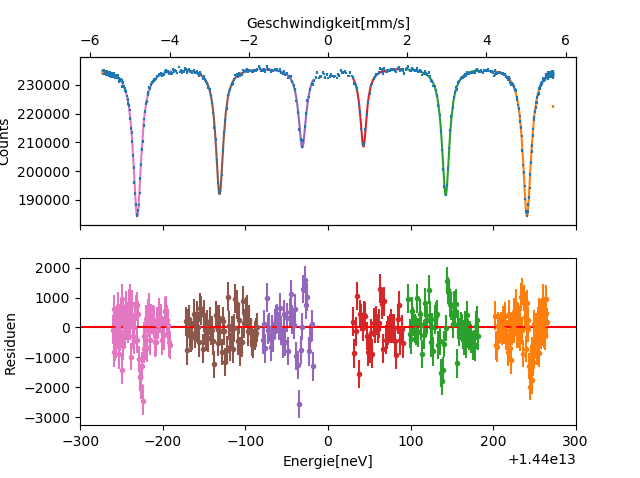
\includegraphics[scale=0.9]{Bilder/Hyperfein/Hyper_fit_nach.png}
\caption{Anpaasungen von quadratischen Funktionen an die Peaks}
\label{fig:Hyper_fit}
\end{figure}

\begin{table}
\centering
\begin{tabular}{|c|c|c|c|c|c|}
\hline
& $I_0$ & b & a & c & $\chi / ndof$\\
\hline
Peak 1 & $ -51658.87 \pm 870.09 $ & $ 234553.56 \pm 103.63 $ & $ -230.17 \pm 0.1 $ & $ 34.76 \pm 1.35 $ & $ 0.462 $\\
\hline
Peak 2& $ -43672.07 \pm 699.54 $ & $ 234203.4 \pm 119.28 $ & $ -129.99 \pm 0.19 $ & $ 30.37 \pm 1.67 $ & $ 0.818 $\\
\hline
Peak 3& $ -28212.83 \pm 1116.91 $ & $ 233753.94 \pm 131.51 $ & $ -30.15 \pm 0.23 $ & $ 28.4 \pm 2.67 $ & $ 0.809 $\\
\hline
Peak 4& $ -26349.96 \pm 268.14 $ & $ 234020.59 \pm 81.22 $ & $ 43.9 \pm 0.15 $ & $ 26.23 \pm 1.24 $ & $ 0.313 $\\
\hline
Peak 5& $ -43843.81 \pm 1473.79 $ & $ 234083.03 \pm 113.84 $ & $ 143.19 \pm 0.17 $ & $ 28.88 \pm 1.94 $ & $ 0.716 $\\
\hline
Peak 6 & $ -51685.83 \pm 430.51 $ & $ 234639.9 \pm 108.89 $ & $ 241.3 \pm 0.09 $ & $ 34.34 \pm 1.02 $ & $ 0.37 $\\
\hline
\end{tabular} 
\caption{Ergebnisse der Anpassungen an das vordere Spektrum. Peaks sind von rechts nach links durchnummeriert.}
\label{tab:Hyper_fit_vor}
\end{table}

\begin{table}
\centering
\begin{tabular}{|c|c|c|c|c|c|}
\hline
& $I_0$ & b & a & c & $\chi / ndof$\\
\hline
Peak 1 & $ -51424.26 \pm 705.82 $ & $ 235692.95 \pm 109.59 $ & $ -231.11 \pm 0.1 $ & $ 35.9 \pm 1.31 $ & $ 0.46 $\\
\hline
Peak 2& $ -43893.01 \pm 1050.77 $ & $ 235892.75 \pm 102.2 $ & $ -131.34 \pm 0.16 $ & $ 31.56 \pm 1.69 $ & $ 0.578 $\\
\hline
Peak 3& $ -27559.47 \pm 778.76 $ & $ 235753.31 \pm 132.76 $ & $ -31.13 \pm 0.23 $ & $ 31.24 \pm 2.51 $ & $ 0.767 $\\
\hline
Peak 4& $ -27182.12 \pm 1325.83 $ & $ 235710.97 \pm 129.38 $ & $ 42.93 \pm 0.24 $ & $ 23.31 \pm 2.49 $ & $ 0.833 $\\
\hline
Peak 5& $ -44249.17 \pm 566.44 $ & $ 235930.07 \pm 112.18 $ & $ 142.59 \pm 0.17 $ & $ 31.59 \pm 1.52 $ & $ 0.675 $\\
\hline
Peak 6 & $ -51531.79 \pm 425.04 $ & $ 235901.73 \pm 101.06 $ & $ 241.04 \pm 0.08 $ & $ 37.53 \pm 1.01 $ & $ 0.308 $\\
\hline
\end{tabular} 
\caption{Ergebnisse der Anpassungen an das hintere Spektrum. Peaks sind von rechts nach links durchnummeriert.}
\label{tab:Hyper_fit_nach}
\end{table}



\begin{table}
\centering
\begin{tabular}{|c|c|c|}
\hline 
$m_g$ & $m_a$ & Peak \\ 
\hline 
1/2 & 3/2 & 1 \\ 
\hline 
1/2 & 1/2 & 2 \\  
\hline 
1/2 & -1/2 & 3 \\ 
\hline 
-1/2 & 1/2 & 4 \\ 
\hline 
-1/2 & -1/2 & 5 \\ 
\hline 
-1/2 & -3/2 & 6 \\ 
\hline 
\end{tabular} 
\caption{Zuordnung der Peaks zu den Drehimpulsen. Die Peaks werden von links (kleinste Energie) nach rechts (größste Energie) durchgezählt. Anmerkung: Es wurde angenommen, dass $\mu_a$ positiv ist. Wenn es negativ ist ändert sich die Reihenfolge.}
\label{tab:Hyper_Zuordnung}
\end{table}

\begin{table}
\centering
\begin{tabular}{|c|c|c|c|}
\hline 
Spektrum & Peaks & Abstand[neV] & Meagnetfeld[T]\\ 
\hline 
vorne & 5-3 & $173.89\pm 0.24$ & $30.57\pm 0.04$\\ 
\hline 
vorne & 4-2 & $173.34\pm 0.29$& $30.47\pm 0.05$\\ 
\hline 
\hline 
hinten & 5-3 & $174.27\pm 0.29$ & $30.63\pm 0.05$\\ 
\hline 
hinten & 4-2 & $173.71\pm 0.29$& $30.54\pm 0.05$\\ 
\hline 
\end{tabular} 
\caption{Energieabstände zur Bestimmung von H.}
\label{tab:Hyper_H}
\end{table}

\begin{table}
\centering
\begin{tabular}{|c|c|c|c|}
\hline 
Spektrum & Peaks & Abstand[neV] & magn. Moment[neVT]\\ 
\hline 
vorne & 2-1 & $100.18 	\pm 0.22$ & $4.91\pm 0.01$\\ 
\hline 
vorne & 3-2 & $99.85\pm 0.29$& $4.90\pm 0.02$\\ 
\hline
vorne & 5-4 & $99.29\pm 0.26$& $4.87\pm 0.01$\\ 
\hline 
vorne & 6-5 & $99.11\pm 0.18$& $4.81\pm 0.01$\\ 
\hline 
\hline 
hinten & 2-1 & $99.84\pm 0.22$ & $4.90\pm 0.01$\\ 
\hline 
hinten & 3-2 & $100.21\pm 0.30$& $4.91\pm 0.02$\\ 
\hline
hinten & 5-4 & $99.66\pm 0.32$& $4.89\pm 0.02$\\ 
\hline 
hinten & 6-5 & $99.45\pm 0.23$& $4.83\pm 0.01$\\ 
\hline 
\end{tabular} 
\caption{Energieabstände zur Bestimmung von $\mu_a$.}
\label{tab:Hyper_mu}
\end{table}

Das Spektrum zur Hyperfeinstrukturaufspaltung ist in Abbildung \ref{fig:Hyper_Roh} dargestellt. Auch hier gibt es die Aufspaltung in 2 gespiegelte Bereiche, welche in Abbildung \ref{fig:Hyper_Data} gegen Geschwindigkeit und Energie kalibriert sind.\\
\\
An die Peaks wird eine Lorentz-Kurve der Form
\begin{equation}
y = I_0 \dfrac{c}{(x-a)^2+c}+b
\end{equation}
angepasst. Dabei ist $I_0$ die maximale Peakhöhe, a die Position in x-Richtung, b die Position in y-Srichtung und c beschreibt die Breite der Kurve.
Die Anpassungen sind in Abbildung \ref{fig:Hyper_fit} dargestellt und die Ergebnisse aus diesen Fits befinden sich in Tabelle \ref{tab:Hyper_fit_vor} für das vordere Spektrum und in Tabelle \ref{tab:Hyper_fit_nach} für das hintere.
\\
Aus den Parameter a der Anpassungen kann man die Abstände zwischen den Peaks bestimmen und so über 
\begin{equation}
\Delta E = -H\left(\dfrac{\mu_a m_a}{j_a}-\dfrac{\mu_g m_g}{j_g}\right)
\label{eq:Hyper}
\end{equation}
das Magnetfeld H und das magnetische Moment $\mu_a$ des angeregten Zusatndes bestimmen. Hier gilt $\mu_g = -2.844\cdot 10^{-9}eVT^{-1}$, $j_a = 3/2$ und $j_g = 1/2$.  Mithilfe dieser Gleichung kann man den Peaks Drehimpulse zuordnen, was in Tabelle \ref{tab:Hyper_Zuordnung} geschehen ist.\\
Die Gleichung hat zwar 2 Unbekannte, durch geschickte Wahl der Peaks, zwischen denen man den Abstand bestimmt, kann man aber $\mu_a$ eliminieren. Dafür müssen zwei Peaks mit gleichem $m_a$ ausgewählt werden. Dies ist nur für Peaks 3/5 und für Peaks 2/4 der Fall. Für diese gilt
\begin{equation}
\Delta E = H\dfrac{\mu_g}{j_g}(m_{5/4}-m_{3/2})
\end{equation}
woraus man direkt H berechnen kann. Dies ist in Tabelle \ref{tab:Hyper_H} geschehen. Der Fehler folgt wieder über gaussche Fehlerfortpflanzung. Eine gewichtete Mittelung ergibt das Endergebnis:
\begin{equation*}
\boxed{H = \SI{30.55\pm 0.03}{T}}
\end{equation*}

\subsubsection{Magentisches Moment}
Um nun das magnetische Moment $\mu_a$ im angeregten Zustand bestimmen zu können werden zwei Peaks mit gleichem $m_g$ ausgewählt und wieder der Abstand zwischen ihnen bestimmt. Dadurch vereinfacht sich Gleichung \ref{eq:Hyper} zu
\begin{equation}
\Delta E = -H\dfrac{\mu_a}{j_a}(m_{a}^i-m_{a}^j)
\end{equation}
woraus man mit bekanntem H das Magentische Moment erhält. Dabei wurden die Peaks 2/1, 3/2 und 5/4, 6/5 betrachtet. Man könnte zwar theoretisch auch Kombinationen über die Spiegelachse (z.B 6/1) betrachten, bei denen aber der hintere Term von Gleichung \ref{eq:Hyper} nicht wegfällt und so die Formel um einiges komplizierter wird.\\
Die so bestimmten Abstände und daraus berechnteten magnetischen Momente sind in Tabelle \ref{tab:Hyper_mu} aufgelistet. Die angegebenen Fehler stammen aus gaussischer Fehlerfortpflanzung der Fehler aus den Fits.\\
Daraus kann man wieder durch gewichtete Mittelung das Endergebnis erhalten:
\begin{equation*}
\boxed{\mu_a = \SI{4.88\pm 0.01}{neVT^{-1}}}
\end{equation*}

\subsubsection{relative Peakhöhe}

Die Intensitäten der Peaks werden über die Beziehung des Anpassungsparameters $c = \gamma^2 = \dfrac{\Gamma^2}{4}$ und die maximale Peakhöhe $I_0$ mithilfe von
\begin{equation}
I_{ges} = \dfrac{I_0 \gamma \pi}{\hbar}
\end{equation}
bestimmt. Man kann also die relativen Intensitäten leicht über
\begin{equation}
\dfrac{I_1}{I_2} = \dfrac{I_0^1 \sqrt{c^1}}{I_0^2 \sqrt{c^2}}
\end{equation}
ausrechnen. Die Fehler folgen durch gaussche Fehlerfortpflanzung aus den Fehlern der Anpassung. Es werden nur Peaks miteinander verglichen, die aus dem selben Teilspektrum stammen, also jeweils nur die Peaks 4,5,6 und 1,2,3.\\
In Tabelle \ref{tab:Hyper_hohe} sind alle relativen Höhe bezogen auf den jeweiligen kleinsten Peak eines Teilspektrums angegeben.\\
\\
Eie gewichtete Mittelung der jeweils zusammengehörenden Peakverhältnisse ergibt ein Verhältnis in der Reihenfolge (Innen : Mitte : Außen) von
\begin{equation}
\boxed{1:(1.69\pm0.09):(2.16\pm0.09)}
\end{equation}
Das Verhältnis zwischen äußerem und mittlerem Peak beträgt demnach $1.28\pm0.08$.
\paragraph{Vergleich mit Erwartung}
Aus der theoretischen Vorhersage hätte man ein Peakverhältnis von 1:2:3 erwartet. Die berechneten Höhenverhältnisse liegen zwar qualitativ in der richtigen Reihenfolge, der innere Peak ist aber im Verhältnis zum mittleren um $13\%$ und zum äußeren um $39\%$ zu groß. Eine Ursache dafür kann sein, dass ein kleiner Teil der Strahlung nicht aufgespalten wird und sich deswegen die inneren Peaks mit dem Einlinienspektrum überlagern. Ein weiterer Hinweis darauf ist, dass die Werte zwischen den beiden inneren Peaks nicht ganz auf die Nullhöhe zurücklaufen, sonder leicht tiefer liegen.\\
Ein weiterer Grund für die Abweichung der Verhältnisse von der Erwartung ist ein nicht ganz unpolarisiertes Magnetfeld, da sich durch Ausrichtung des Feldes die relativen Höhen ändern.

\begin{table}
\centering
\begin{tabular}{|c|c|c|}
\hline 
Spektrum & Peaks & rel. Höhe\\ 
\hline 
vorne & 2/3 & $1.74\pm 0.16$\\ 
\hline 
vorne & 5/4 & $1.60\pm 0.19$\\ 
\hline
hinten & 2/3 & $1.89\pm 0.24$\\ 
\hline
hinten & 5/4 & $1.60\pm 0.17$\\ 
\hline
\hline
vorne & 1/3 & $2.24\pm 0.13$\\ 
\hline
vorne & 6/4 & $2.03\pm 0.22$\\ 
\hline 
hinten & 1/3 & $2.41\pm 0.29$\\ 
\hline
hinten & 6/4 & $2.00\pm 0.19$\\ 
\hline
\end{tabular} 
\caption{Relative Peakhöhen bezogen auf die kleinsten Peaks (3 und 4). Der obere Teil beschreibt die relative Höhe zwischen kleinstem und mittleren Peak und der untere Teil die Höhe zwischen kleinstem und größten Peak.}
\label{tab:Hyper_hohe}
\end{table}

\subsubsection{Isomerieverschiebung}
\begin{table}
\centering
\begin{tabular}{|c|c|c|}
\hline 
Spektrum & Peaks & Mittelpunkt \\ 
\hline 
vorne & 3 und 4 & $6.88\pm 0.31$ \\ 
\hline 
vorne & 2 und 5 & $6.60\pm 0.30$ \\ 
\hline 
vorne & 1 und 6 & $5.56\pm 0.22$ \\ 
\hline
\hline
hinten & 3 und 4 & $5.90\pm 0.34$ \\ 
\hline 
hinten & 2 und 5 & $5.62\pm 0.29$ \\ 
\hline 
hinten & 1 und 6 & $4.97\pm 0.21$ \\ 
\hline 
\end{tabular} 
\caption{Mittelpunkte zwischen den jeweiligen symmetrischen Peaks zur Bestimmung der Isomerieverschieung.}
\label{tab:Hyper_Iso}
\end{table}

Die Isomerieverschiebung wird hier über den Mittelpunkt zwischen 2 symmetrischen Peaks bestimmt, da diese die geliche Energieaufspaltung bestitzen sollten. Aus dem gewichteten Mittel dieser Verschiebungen erhält man die Isomerieverschiebung:
\begin{equation*}
\boxed{\delta = \SI{5.74\pm 0.29}{neV}}
\end{equation*}


\subsection{Elektrische Quadrupolaufspaltung}

\subsubsection{Quadrupolmoment}

\begin{figure}
\centering
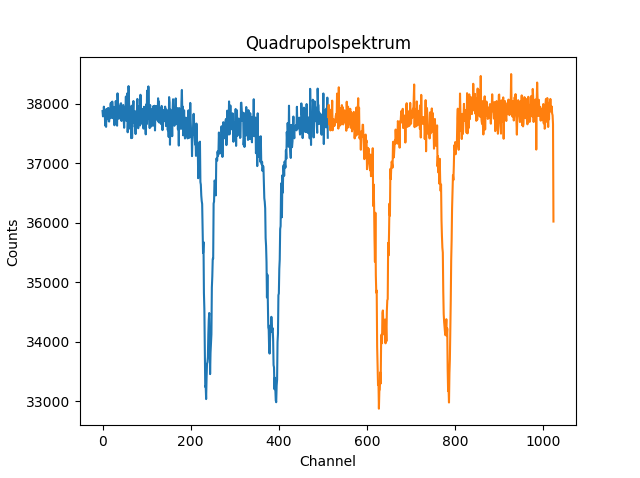
\includegraphics[scale=0.8]{Bilder/Quadrupol/Quad_Roh.png}
\caption{Quadrupolaufspaltung Rohdaten}
\label{fig:Quad_Roh}
\end{figure}

\begin{figure}
\centering
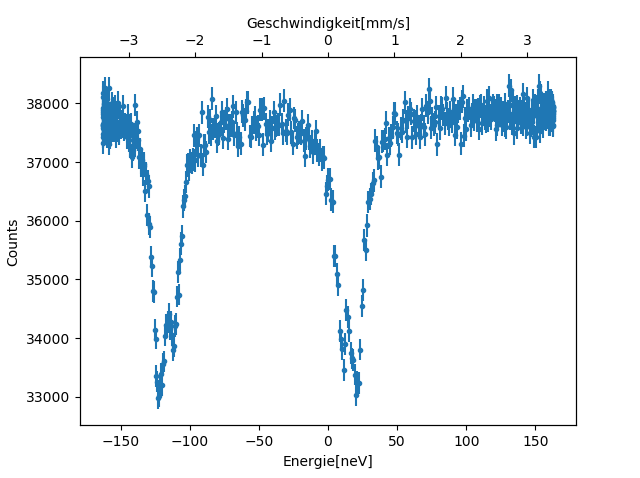
\includegraphics[scale=0.8]{Bilder/Quadrupol/Quad_Data_vor.png}
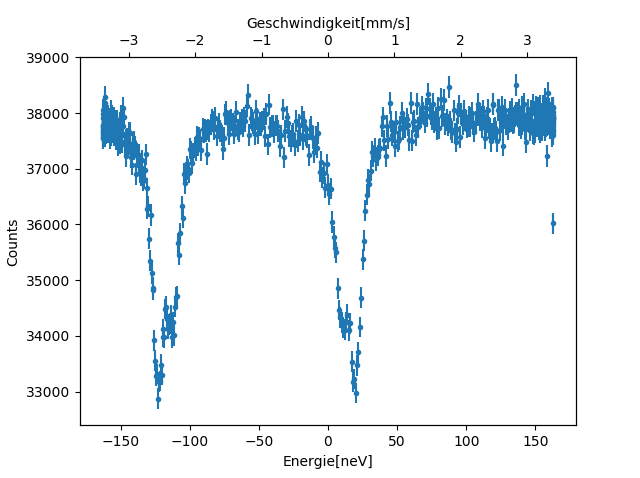
\includegraphics[scale=0.8]{Bilder/Quadrupol/Quad_Data_nach.png}
\caption{Quadrupolaufspaltung gegen Energie und Geschwindigkeit.}
\label{fig:Quad_Data}
\end{figure}

\begin{figure}
\centering
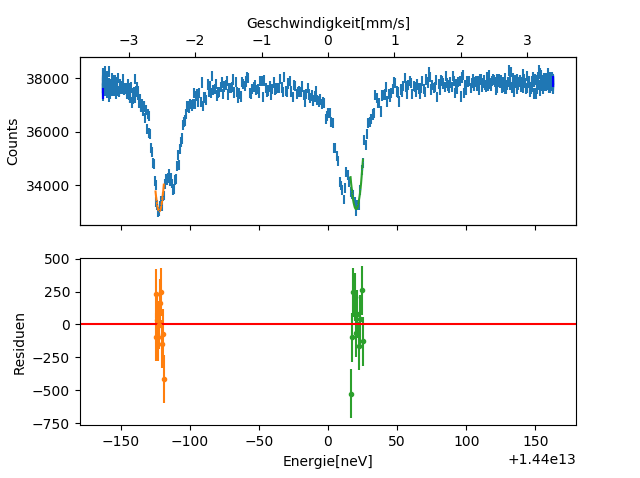
\includegraphics[scale=0.8]{Bilder/Quadrupol/Quad_fit_vor.png}
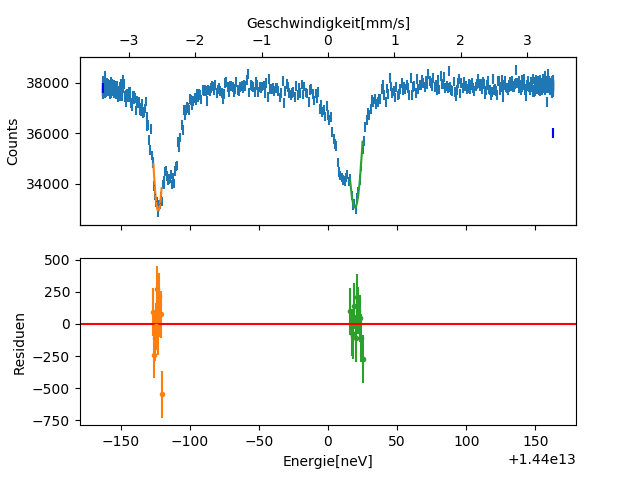
\includegraphics[scale=0.8]{Bilder/Quadrupol/Quad_fit_nach.png}
\caption{Quadratische Anpassung an die Umgebungen der Peaks.}
\label{fig:Quad_fit}
\end{figure}

Das gemessene Spektrum ist in Abbildung \ref{fig:Quad_Roh} dargestellt, die Aufspaltung in die beiden Bereiche und die Darstellung mit Geschwindigkeit- und Energieachse in Abbildung \ref{fig:Quad_Data}.\\
Mithilfe von 2 quadratischen Anpassungen der Form
\begin{equation}
y = a(x-b)^2+c
\end{equation}
wird die Peakposition bestimmt. Diese sind in Abbildung \ref{fig:Quad_fit} zu sehen. In Tabelle \ref{tab:Quad_vor} sind die Ergebnisse der Anpassungen zu finden.\\
\\
Aus dem Fitparameter b kann man nun die Energieposition und daraus die Energiedifferenz der beiden Peaks bestimmt werden. Mithilfe der Gleichung
\begin{equation}
\Delta E = \dfrac{1}{4 \pi \epsilon_0}\dfrac{4}{7}(1-R)^2e^2\cdot Q \cdot \left(\dfrac{1}{r^3}\right)_{3d}
\label{eq:Quad}
\end{equation}
kann das Quadrupolmoment Q bestimmt werden, wobei $R = 0.42$ und $(r^{-3})_{3d} = 35\cdot 10^{24} cm^{-3}$. Die Ergebnisse sind in Tabelle \ref{tab:Quad_ergebnis} aufgelistet.\\
Der gewichtete Mittelwert ergibt für das Quadrupolmoment:
\begin{equation*}
\boxed{Q = \SI{8.52\pm 0.01}{fm^2}}
\end{equation*}

\paragraph{Vergleich mit Literaturwert}
Der Literaturwert des Quadrupolmomentes beträgt $\SI{18}{fm^2}$. Unser gemessener Wert ist also um einen Faktor 2.1 zu klein. Dies liegt vermutlich daran, dass Gleichung \ref{eq:Quad} nur für tiefe Temperaturen gilt. Es wurde aber bei Raumtemperatur gearbeitet.


\begin{table}
\centering
\begin{tabular}{|c|c|c|c|c|c|}
\hline
Spektrum &  & a & b & c & $\chi / ndof$\\
\hline
vorne & Peak 1 & $ 96.9 \pm 24.53 $ & $ -121.93 \pm 0.21 $ & $ 33013.17 \pm 67.48 $ & $ 0.294 $\\
\hline
vorne & Peak 2& $ 74.5 \pm 13.76 $ & $ 20.31 \pm 0.24 $ & $ 33098.98 \pm 80.66 $ & $ 0.379 $\\
\hline
\hline
hinten & Peak 1& $ 153.99 \pm 36.93 $ & $ -122.73 \pm 0.2 $ & $ 32928.74 \pm 85.57 $ & $ 0.282 $\\
\hline
hinten & Peak 2& $ 86.68 \pm 11.15 $ & $ 19.51 \pm 0.18 $ & $ 33066.82 \pm 59.87 $ & $ 0.198 $\\
\hline
\end{tabular}
\caption{Ergebnsse der Anpassungen.}
\label{tab:Quad_vor}
\end{table}

\begin{table}
\centering
\begin{tabular}{|c|c|c|}
\hline
Spektrum & Abstand[neV] & Quadrupolmoment[$\si{fm^2}$]\\
\hline
vorne & $ 142.23 \pm 0.32 $ & $ 8.515 \pm 0.019 $\\
\hline
\hline
hinten & $ 142.24 \pm 0.27 $ & $ 8.516 \pm 0.016 $\\
\hline
\end{tabular}
\caption{Ergebnsse der Anpassungen.}
\label{tab:Quad_ergebnis}
\end{table}

\subsubsection{Isomerieverschiebung}
Über den Mittelpunkt zwischen den beiden Peaks kann man auch hier die Isomerieverscheibung bestimmen. Die Ergebnisse sind in Tabelle \ref{tab:Quad_Iso} aufgelistet, wobei die Fehler gaussisch aus den Anpassungsfehlern fortgepflanzt wurden. Der gewichtete Mittelwert ergibt
\begin{equation*}
\boxed{\delta = \SI{-51.27\pm 0.40}{neV}}
\end{equation*}

\begin{table}
\centering
\begin{tabular}{|c|c|}
\hline
Spektrum & Isomerieverschiebung[neV]\\
\hline
vorne & $ -50.81\pm 0.34 $\\
\hline
\hline
hinten & $ -51.61 \pm 0.31 $\\
\hline
\end{tabular}
\caption{Isomerieverschiebung im Spektum vom Quadrupolmoment}
\label{tab:Quad_Iso}
\end{table}

\section{Fazit}


\newpage
\section{Anhang}
\subsection{Kalibration}
\begin{figure} [H]
\centering
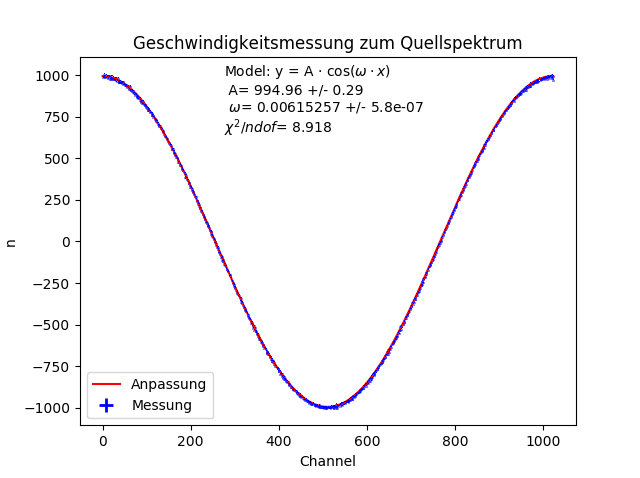
\includegraphics[scale=0.8]{Bilder/Kalibration/Quellspektrum.png}
\caption{Aufnahme zur Geschwindigkeits- und Energiekalibration vor der Messung des Quellspektrums.}
\end{figure}

\begin{figure} [H]
\centering
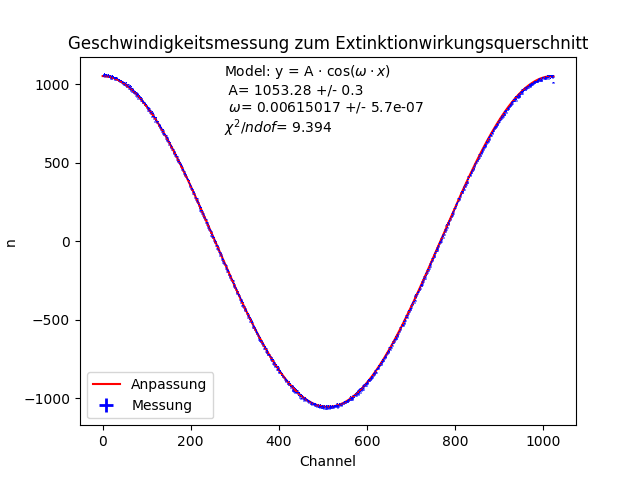
\includegraphics[scale=0.8]{Bilder/Kalibration/Extinktion.png}
\caption{Aufnahme zur Geschwindigkeits- und Energiekalibration vor der Messung des Extinktionswirkungsquerschnitts.}
\end{figure}

\begin{figure} [H]
\centering
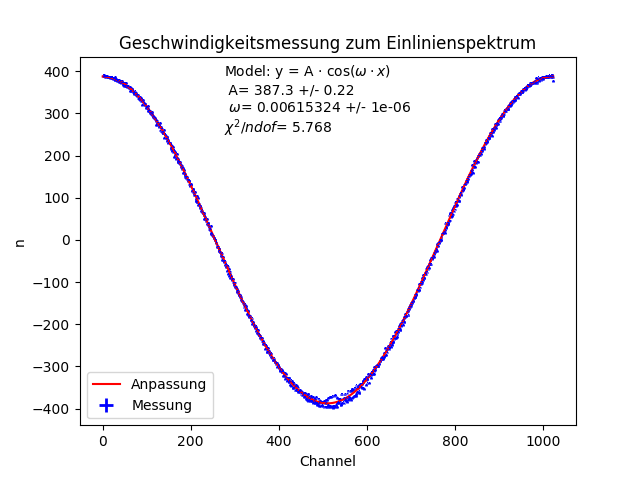
\includegraphics[scale=0.8]{Bilder/Kalibration/Einlinien.png}
\caption{Aufnahme zur Geschwindigkeits- und Energiekalibration vor der Messung des Einlinienspektrums.}
\end{figure}

\begin{figure} [H]
\centering
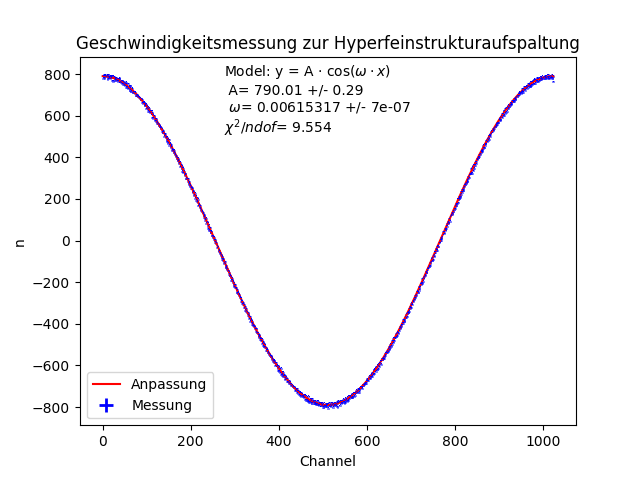
\includegraphics[scale=0.8]{Bilder/Kalibration/Hyperfein.png}
\caption{Aufnahme zur Geschwindigkeits- und Energiekalibration vor der Messung der magnetischen Hyperfeinstrukturaufspaltung.}
\end{figure}

\begin{figure} [H]
\centering
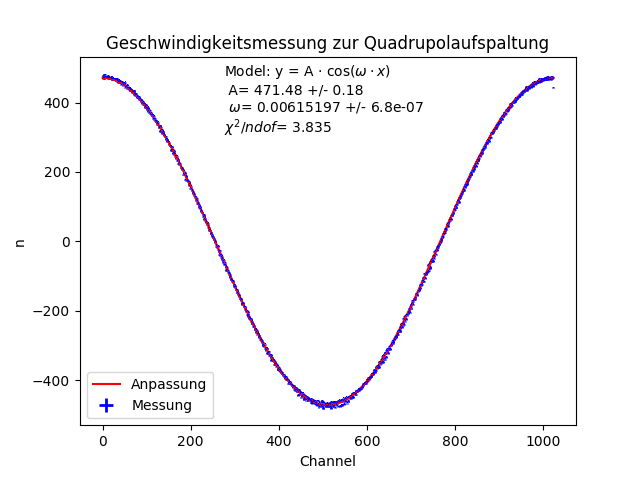
\includegraphics[scale=0.8]{Bilder/Kalibration/Quadrupol.png}
\caption{Aufnahme zur Geschwindigkeits- und Energiekalibration vor der Messung der elektrischen Quadrupolaufspaltung.}
\end{figure}

\subsection{Untergrundmessung}
\begin{figure} [H]
\centering
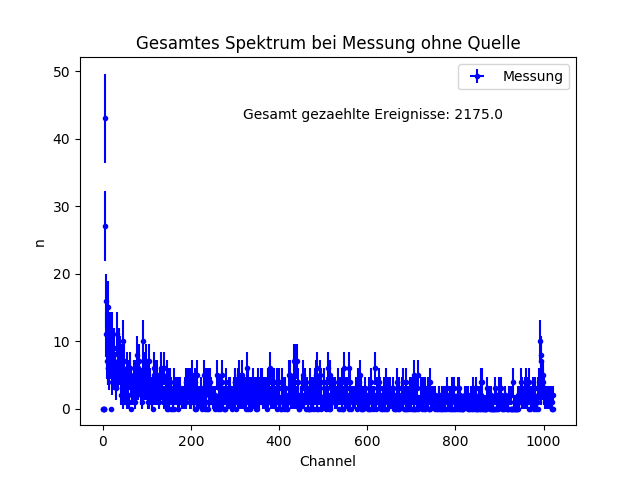
\includegraphics[scale=0.8]{Bilder/Extinktion/Rauschmessung.png}
\caption{Untergrundmessung ohne Quelle und ohne Absorber zur Korrektur bei den Messungen zum Extinktionswirkungsquerschnitt.}
\end{figure}

\subsection{Extinktionswirkungsquerschnitt}
\begin{figure} [H]
\centering
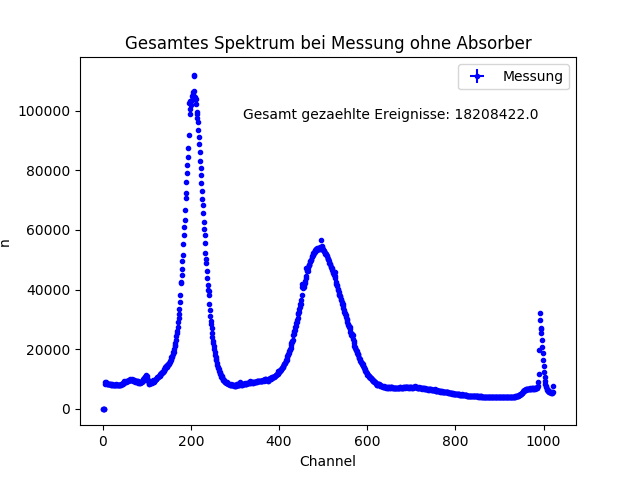
\includegraphics[scale=0.8]{Bilder/Extinktion/OhneAbsorber.png}
\caption{Messung des Spektrums ohne Absorber zur Bestimmung des Extinktionwirkungsquerschnitts.}
\end{figure}

\begin{figure} [H]
\centering
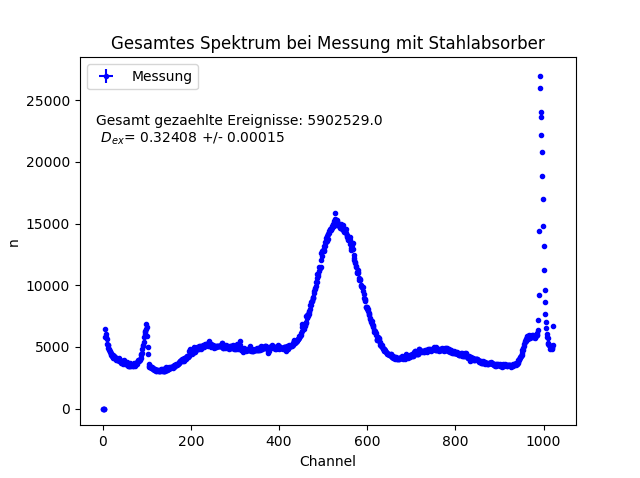
\includegraphics[scale=0.8]{Bilder/Extinktion/Stahl.png}
\caption{Messung des Spektrums zur Bestimmung des Extinktionwirkungsquerschnitts von Stahl.}
\end{figure}

\begin{figure} [H]
\centering
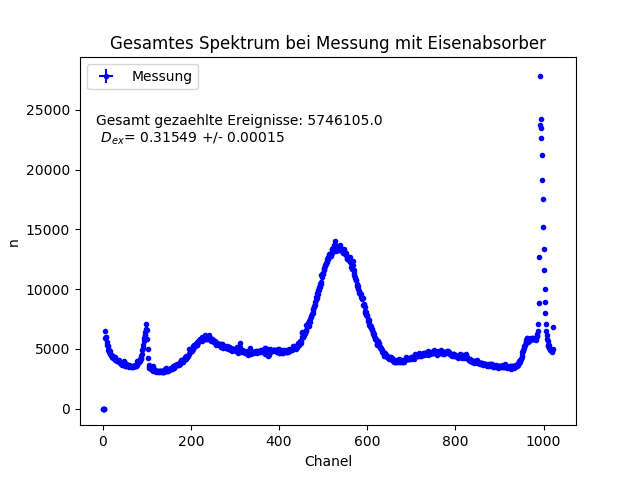
\includegraphics[scale=0.8]{Bilder/Extinktion/Eisen.png}
\caption{Messung des Spektrums zur Bestimmung des Extinktionwirkungsquerschnitts von reinem Eisen.}
\end{figure}

\begin{figure} [H]
\centering
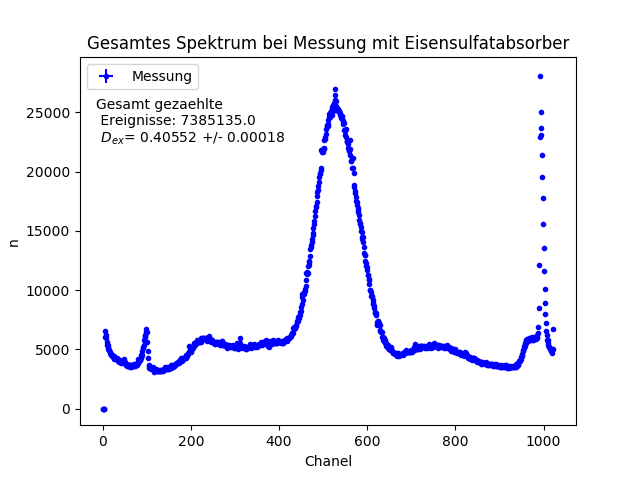
\includegraphics[scale=0.8]{Bilder/Extinktion/Eisensulfat.png}
\caption{Messung des Spektrums zur Bestimmung des Extinktionwirkungsquerschnitts von FeSO$_4$ $\cdot$ 7H$_2$O.}
\end{figure}

\subsection{Quellenspektrum}
\subsection{Einlinienspektrum}
\subsection{Magnetische Hyperfeinstrukturaufspaltung}
\subsection{Elektrische Quadrupolaufspaltung}


\end{document}
